\batchmode
\documentclass[twoside]{book}

% Packages required by doxygen
\usepackage{fixltx2e}
\usepackage{calc}
\usepackage{doxygen}
\usepackage[export]{adjustbox} % also loads graphicx
\usepackage{graphicx}
\usepackage[utf8]{inputenc}
\usepackage{makeidx}
\usepackage{multicol}
\usepackage{multirow}
\PassOptionsToPackage{warn}{textcomp}
\usepackage{textcomp}
\usepackage[nointegrals]{wasysym}
\usepackage[table]{xcolor}

% Font selection
\usepackage[T1]{fontenc}
\usepackage[scaled=.90]{helvet}
\usepackage{courier}
\usepackage{amssymb}
\usepackage{sectsty}
\renewcommand{\familydefault}{\sfdefault}
\allsectionsfont{%
  \fontseries{bc}\selectfont%
  \color{darkgray}%
}
\renewcommand{\DoxyLabelFont}{%
  \fontseries{bc}\selectfont%
  \color{darkgray}%
}
\newcommand{\+}{\discretionary{\mbox{\scriptsize$\hookleftarrow$}}{}{}}

% Page & text layout
\usepackage{geometry}
\geometry{%
  a4paper,%
  top=2.5cm,%
  bottom=2.5cm,%
  left=2.5cm,%
  right=2.5cm%
}
\tolerance=750
\hfuzz=15pt
\hbadness=750
\setlength{\emergencystretch}{15pt}
\setlength{\parindent}{0cm}
\setlength{\parskip}{3ex plus 2ex minus 2ex}
\makeatletter
\renewcommand{\paragraph}{%
  \@startsection{paragraph}{4}{0ex}{-1.0ex}{1.0ex}{%
    \normalfont\normalsize\bfseries\SS@parafont%
  }%
}
\renewcommand{\subparagraph}{%
  \@startsection{subparagraph}{5}{0ex}{-1.0ex}{1.0ex}{%
    \normalfont\normalsize\bfseries\SS@subparafont%
  }%
}
\makeatother

% Headers & footers
\usepackage{fancyhdr}
\pagestyle{fancyplain}
\fancyhead[LE]{\fancyplain{}{\bfseries\thepage}}
\fancyhead[CE]{\fancyplain{}{}}
\fancyhead[RE]{\fancyplain{}{\bfseries\leftmark}}
\fancyhead[LO]{\fancyplain{}{\bfseries\rightmark}}
\fancyhead[CO]{\fancyplain{}{}}
\fancyhead[RO]{\fancyplain{}{\bfseries\thepage}}
\fancyfoot[LE]{\fancyplain{}{}}
\fancyfoot[CE]{\fancyplain{}{}}
\fancyfoot[RE]{\fancyplain{}{\bfseries\scriptsize Generated by Doxygen }}
\fancyfoot[LO]{\fancyplain{}{\bfseries\scriptsize Generated by Doxygen }}
\fancyfoot[CO]{\fancyplain{}{}}
\fancyfoot[RO]{\fancyplain{}{}}
\renewcommand{\footrulewidth}{0.4pt}
\renewcommand{\chaptermark}[1]{%
  \markboth{#1}{}%
}
\renewcommand{\sectionmark}[1]{%
  \markright{\thesection\ #1}%
}

% Indices & bibliography
\usepackage{natbib}
\usepackage[titles]{tocloft}
\setcounter{tocdepth}{3}
\setcounter{secnumdepth}{5}
\makeindex

% Hyperlinks (required, but should be loaded last)
\usepackage{ifpdf}
\ifpdf
  \usepackage[pdftex,pagebackref=true]{hyperref}
\else
  \usepackage[ps2pdf,pagebackref=true]{hyperref}
\fi
\hypersetup{%
  colorlinks=true,%
  linkcolor=blue,%
  citecolor=blue,%
  unicode%
}

% Custom commands
\newcommand{\clearemptydoublepage}{%
  \newpage{\pagestyle{empty}\cleardoublepage}%
}

\usepackage{caption}
\captionsetup{labelsep=space,justification=centering,font={bf},singlelinecheck=off,skip=4pt,position=top}

%===== C O N T E N T S =====

\begin{document}

% Titlepage & ToC
\hypersetup{pageanchor=false,
             bookmarksnumbered=true,
             pdfencoding=unicode
            }
\pagenumbering{alph}
\pagenumbering{arabic}
\hypersetup{pageanchor=true}

%--- Begin generated contents ---
\chapter{Demo problem\+: Adaptive solution of Poisson\textquotesingle{}s equation in a fish-\/shaped domain.}
\label{index}\hypertarget{index}{}\hypertarget{index_q}{}\section{A few quick questions...}\label{index_q}
Since {\ttfamily oomph-\/lib} is developed as open-\/source software, any evidence that the code is being downloaded and used is very helpful for us as it helps to justify our continued work on this project.

We would therefore be extremely grateful if you could provide the information requested in the form below. Pressing the \char`\"{}submit\char`\"{} button will get you to the actual download page.

{\bfseries Note\+:} 
\begin{DoxyItemize}
\item All information will be treated as confidential. 
\item If you provide your email address and check the appropriate box we will add you to our mailing list to inform you of upgrades and bug fixes to the code. Rest assured that the mailing list is {\bfseries very low volume} -- we have better things to do than to bombard you with email. 
\item If you still feel reluctant to provide any of the information requested, feel free to enter some dummy input. The form will check that {\bfseries some} information has been entered but entering your name as \char`\"{}\+Joe Cool\char`\"{} is perfectly acceptable -- this is to discourage people from not providing the information simply because they are too lazy to type... 
\end{DoxyItemize}



 







 

 \hypertarget{index_pdf}{}\section{P\+D\+F file}\label{index_pdf}
A \href{../latex/refman.pdf}{\tt pdf version} of this document is available. \end{document}

\chapter{Namespace Index}
\section{Namespace List}
Here is a list of all namespaces with brief descriptions\+:\begin{DoxyCompactList}
\item\contentsline{section}{\hyperlink{namespaceGlobal__Physical__Variables}{Global\+\_\+\+Physical\+\_\+\+Variables} \\*Global variables that represent physical properties }{\pageref{namespaceGlobal__Physical__Variables}}{}
\item\contentsline{section}{\hyperlink{namespaceoomph}{oomph} }{\pageref{namespaceoomph}}{}
\item\contentsline{section}{\hyperlink{namespacePhysical__Variables}{Physical\+\_\+\+Variables} \\*Namespace for the solution of 2D linear shell equation }{\pageref{namespacePhysical__Variables}}{}
\end{DoxyCompactList}

\chapter{Hierarchical Index}
\section{Class Hierarchy}
This inheritance list is sorted roughly, but not completely, alphabetically\+:\begin{DoxyCompactList}
\item Problem\begin{DoxyCompactList}
\item \contentsline{section}{Unstructured\+Solid\+Problem$<$ E\+L\+E\+M\+E\+NT $>$}{\pageref{classUnstructuredSolidProblem}}{}
\end{DoxyCompactList}
\end{DoxyCompactList}

\chapter{Class Index}
\section{Class List}
Here are the classes, structs, unions and interfaces with brief descriptions\+:\begin{DoxyCompactList}
\item\contentsline{section}{\hyperlink{classPMLProblem}{P\+M\+L\+Problem$<$ E\+L\+E\+M\+E\+N\+T $>$} }{\pageref{classPMLProblem}}{}
\item\contentsline{section}{\hyperlink{classGlobalParameters_1_1TestPMLMapping}{Global\+Parameters\+::\+Test\+P\+M\+L\+Mapping} }{\pageref{classGlobalParameters_1_1TestPMLMapping}}{}
\end{DoxyCompactList}

\chapter{File Index}
\section{File List}
Here is a list of all files with brief descriptions\+:\begin{DoxyCompactList}
\item\contentsline{section}{\hyperlink{jeffery__orbit_8cc}{jeffery\+\_\+orbit.\+cc} }{\pageref{jeffery__orbit_8cc}}{}
\item\contentsline{section}{\hyperlink{jeffery__orbit_8txt__doxygenified_8h}{jeffery\+\_\+orbit.\+txt\+\_\+doxygenified.\+h} }{\pageref{jeffery__orbit_8txt__doxygenified_8h}}{}
\item\contentsline{section}{\hyperlink{my__taylor__hood__elements_8h}{my\+\_\+taylor\+\_\+hood\+\_\+elements.\+h} }{\pageref{my__taylor__hood__elements_8h}}{}
\end{DoxyCompactList}

\chapter{Namespace Documentation}
\hypertarget{namespaceConstSourceForPoisson}{}\section{Const\+Source\+For\+Poisson Namespace Reference}
\label{namespaceConstSourceForPoisson}\index{Const\+Source\+For\+Poisson@{Const\+Source\+For\+Poisson}}


Namespace for const source term in Poisson equation.  


\subsection*{Functions}
\begin{DoxyCompactItemize}
\item 
void \hyperlink{namespaceConstSourceForPoisson_aeaa1153817bde9598372b803342f3299}{source\+\_\+function} (const Vector$<$ double $>$ \&x, double \&source)
\begin{DoxyCompactList}\small\item\em Const source function. \end{DoxyCompactList}\end{DoxyCompactItemize}
\subsection*{Variables}
\begin{DoxyCompactItemize}
\item 
double \hyperlink{namespaceConstSourceForPoisson_add351c5acab2561d68d1fc9ec3d5fc5e}{Strength} =-\/1.\+0
\begin{DoxyCompactList}\small\item\em Strength of source function\+: default value -\/1.\+0. \end{DoxyCompactList}\end{DoxyCompactItemize}


\subsection{Detailed Description}
Namespace for const source term in Poisson equation. 

\subsection{Function Documentation}
\mbox{\Hypertarget{namespaceConstSourceForPoisson_aeaa1153817bde9598372b803342f3299}\label{namespaceConstSourceForPoisson_aeaa1153817bde9598372b803342f3299}} 
\index{Const\+Source\+For\+Poisson@{Const\+Source\+For\+Poisson}!source\+\_\+function@{source\+\_\+function}}
\index{source\+\_\+function@{source\+\_\+function}!Const\+Source\+For\+Poisson@{Const\+Source\+For\+Poisson}}
\subsubsection{\texorpdfstring{source\+\_\+function()}{source\_function()}}
{\footnotesize\ttfamily void Const\+Source\+For\+Poisson\+::source\+\_\+function (\begin{DoxyParamCaption}\item[{const Vector$<$ double $>$ \&}]{x,  }\item[{double \&}]{source }\end{DoxyParamCaption})}



Const source function. 



Definition at line 58 of file fish\+\_\+poisson.\+cc.



References Strength.



Referenced by Fish\+Poisson\+Problem$<$ E\+L\+E\+M\+E\+N\+T $>$\+::\+Fish\+Poisson\+Problem(), and Refineable\+Fish\+Poisson\+Problem$<$ E\+L\+E\+M\+E\+N\+T $>$\+::\+Refineable\+Fish\+Poisson\+Problem().



\subsection{Variable Documentation}
\mbox{\Hypertarget{namespaceConstSourceForPoisson_add351c5acab2561d68d1fc9ec3d5fc5e}\label{namespaceConstSourceForPoisson_add351c5acab2561d68d1fc9ec3d5fc5e}} 
\index{Const\+Source\+For\+Poisson@{Const\+Source\+For\+Poisson}!Strength@{Strength}}
\index{Strength@{Strength}!Const\+Source\+For\+Poisson@{Const\+Source\+For\+Poisson}}
\subsubsection{\texorpdfstring{Strength}{Strength}}
{\footnotesize\ttfamily double Const\+Source\+For\+Poisson\+::\+Strength =-\/1.\+0}



Strength of source function\+: default value -\/1.\+0. 



Definition at line 55 of file fish\+\_\+poisson.\+cc.



Referenced by source\+\_\+function().


\chapter{Class Documentation}
\hypertarget{classFishPoissonProblem}{}\section{Fish\+Poisson\+Problem$<$ E\+L\+E\+M\+E\+NT $>$ Class Template Reference}
\label{classFishPoissonProblem}\index{Fish\+Poisson\+Problem$<$ E\+L\+E\+M\+E\+N\+T $>$@{Fish\+Poisson\+Problem$<$ E\+L\+E\+M\+E\+N\+T $>$}}
Inheritance diagram for Fish\+Poisson\+Problem$<$ E\+L\+E\+M\+E\+NT $>$\+:\begin{figure}[H]
\begin{center}
\leavevmode
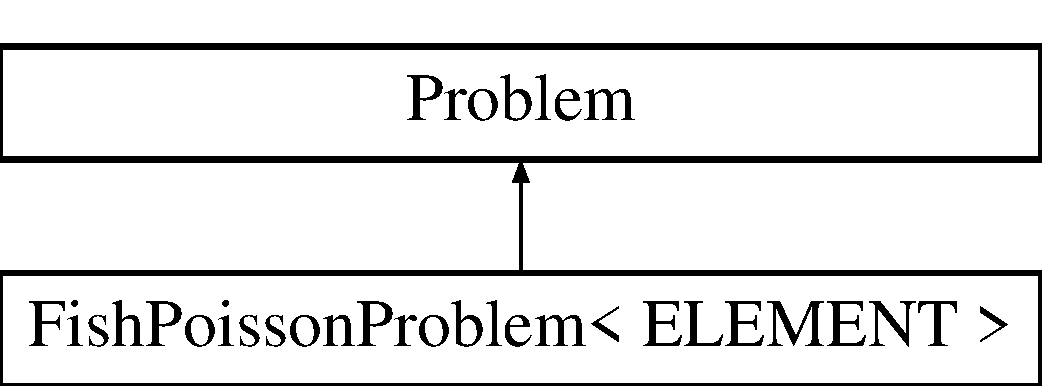
\includegraphics[height=2.000000cm]{classFishPoissonProblem}
\end{center}
\end{figure}
\subsection*{Public Member Functions}
\begin{DoxyCompactItemize}
\item 
\hyperlink{classFishPoissonProblem_ab283ed2dc6985c2871afb09d96b0cff0}{Fish\+Poisson\+Problem} ()
\begin{DoxyCompactList}\small\item\em Constructor. \end{DoxyCompactList}\item 
virtual \hyperlink{classFishPoissonProblem_ad4e0b221af80c3bcc77badc40657a385}{$\sim$\+Fish\+Poisson\+Problem} ()
\begin{DoxyCompactList}\small\item\em Destructor\+: Empty. \end{DoxyCompactList}\item 
void \hyperlink{classFishPoissonProblem_a76f4ada436ceaa1d0ba96289503d99aa}{actions\+\_\+after\+\_\+newton\+\_\+solve} ()
\begin{DoxyCompactList}\small\item\em Update the problem specs after solve (empty) \end{DoxyCompactList}\item 
void \hyperlink{classFishPoissonProblem_a4f3ddd6ae8117d36cace040a2cad68a3}{actions\+\_\+before\+\_\+newton\+\_\+solve} ()
\begin{DoxyCompactList}\small\item\em Update the problem specs before solve (empty) \end{DoxyCompactList}\item 
Fish\+Mesh$<$ E\+L\+E\+M\+E\+NT $>$ $\ast$ \hyperlink{classFishPoissonProblem_a084fca53b2a82803d07326ba27af75ec}{mesh\+\_\+pt} ()
\begin{DoxyCompactList}\small\item\em Overloaded version of the problem\textquotesingle{}s access function to the mesh. Recasts the pointer to the base Mesh object to the actual mesh type. \end{DoxyCompactList}\item 
void \hyperlink{classFishPoissonProblem_a728ae67316d80029132b98b6a4e5ffe5}{doc\+\_\+solution} (Doc\+Info \&doc\+\_\+info)
\begin{DoxyCompactList}\small\item\em Doc the solution. Output directory and labels are specified by Doc\+Info object. \end{DoxyCompactList}\end{DoxyCompactItemize}


\subsection{Detailed Description}
\subsubsection*{template$<$class E\+L\+E\+M\+E\+NT$>$\newline
class Fish\+Poisson\+Problem$<$ E\+L\+E\+M\+E\+N\+T $>$}

Poisson problem in fish-\/shaped domain. Template parameter identifies the element type. 

Definition at line 71 of file fish\+\_\+poisson\+\_\+no\+\_\+adapt.\+cc.



\subsection{Constructor \& Destructor Documentation}
\mbox{\Hypertarget{classFishPoissonProblem_ab283ed2dc6985c2871afb09d96b0cff0}\label{classFishPoissonProblem_ab283ed2dc6985c2871afb09d96b0cff0}} 
\index{Fish\+Poisson\+Problem@{Fish\+Poisson\+Problem}!Fish\+Poisson\+Problem@{Fish\+Poisson\+Problem}}
\index{Fish\+Poisson\+Problem@{Fish\+Poisson\+Problem}!Fish\+Poisson\+Problem@{Fish\+Poisson\+Problem}}
\subsubsection{\texorpdfstring{Fish\+Poisson\+Problem()}{FishPoissonProblem()}}
{\footnotesize\ttfamily template$<$class E\+L\+E\+M\+E\+NT $>$ \\
\hyperlink{classFishPoissonProblem}{Fish\+Poisson\+Problem}$<$ E\+L\+E\+M\+E\+NT $>$\+::\hyperlink{classFishPoissonProblem}{Fish\+Poisson\+Problem} (\begin{DoxyParamCaption}{ }\end{DoxyParamCaption})}



Constructor. 

Constructor for Poisson problem in fish-\/shaped domain. 

Definition at line 111 of file fish\+\_\+poisson\+\_\+no\+\_\+adapt.\+cc.



References Const\+Source\+For\+Poisson\+::source\+\_\+function().

\mbox{\Hypertarget{classFishPoissonProblem_ad4e0b221af80c3bcc77badc40657a385}\label{classFishPoissonProblem_ad4e0b221af80c3bcc77badc40657a385}} 
\index{Fish\+Poisson\+Problem@{Fish\+Poisson\+Problem}!````~Fish\+Poisson\+Problem@{$\sim$\+Fish\+Poisson\+Problem}}
\index{````~Fish\+Poisson\+Problem@{$\sim$\+Fish\+Poisson\+Problem}!Fish\+Poisson\+Problem@{Fish\+Poisson\+Problem}}
\subsubsection{\texorpdfstring{$\sim$\+Fish\+Poisson\+Problem()}{~FishPoissonProblem()}}
{\footnotesize\ttfamily template$<$class E\+L\+E\+M\+E\+NT$>$ \\
virtual \hyperlink{classFishPoissonProblem}{Fish\+Poisson\+Problem}$<$ E\+L\+E\+M\+E\+NT $>$\+::$\sim$\hyperlink{classFishPoissonProblem}{Fish\+Poisson\+Problem} (\begin{DoxyParamCaption}{ }\end{DoxyParamCaption})\hspace{0.3cm}{\ttfamily [inline]}, {\ttfamily [virtual]}}



Destructor\+: Empty. 



Definition at line 80 of file fish\+\_\+poisson\+\_\+no\+\_\+adapt.\+cc.



\subsection{Member Function Documentation}
\mbox{\Hypertarget{classFishPoissonProblem_a76f4ada436ceaa1d0ba96289503d99aa}\label{classFishPoissonProblem_a76f4ada436ceaa1d0ba96289503d99aa}} 
\index{Fish\+Poisson\+Problem@{Fish\+Poisson\+Problem}!actions\+\_\+after\+\_\+newton\+\_\+solve@{actions\+\_\+after\+\_\+newton\+\_\+solve}}
\index{actions\+\_\+after\+\_\+newton\+\_\+solve@{actions\+\_\+after\+\_\+newton\+\_\+solve}!Fish\+Poisson\+Problem@{Fish\+Poisson\+Problem}}
\subsubsection{\texorpdfstring{actions\+\_\+after\+\_\+newton\+\_\+solve()}{actions\_after\_newton\_solve()}}
{\footnotesize\ttfamily template$<$class E\+L\+E\+M\+E\+NT$>$ \\
void \hyperlink{classFishPoissonProblem}{Fish\+Poisson\+Problem}$<$ E\+L\+E\+M\+E\+NT $>$\+::actions\+\_\+after\+\_\+newton\+\_\+solve (\begin{DoxyParamCaption}{ }\end{DoxyParamCaption})\hspace{0.3cm}{\ttfamily [inline]}}



Update the problem specs after solve (empty) 



Definition at line 83 of file fish\+\_\+poisson\+\_\+no\+\_\+adapt.\+cc.

\mbox{\Hypertarget{classFishPoissonProblem_a4f3ddd6ae8117d36cace040a2cad68a3}\label{classFishPoissonProblem_a4f3ddd6ae8117d36cace040a2cad68a3}} 
\index{Fish\+Poisson\+Problem@{Fish\+Poisson\+Problem}!actions\+\_\+before\+\_\+newton\+\_\+solve@{actions\+\_\+before\+\_\+newton\+\_\+solve}}
\index{actions\+\_\+before\+\_\+newton\+\_\+solve@{actions\+\_\+before\+\_\+newton\+\_\+solve}!Fish\+Poisson\+Problem@{Fish\+Poisson\+Problem}}
\subsubsection{\texorpdfstring{actions\+\_\+before\+\_\+newton\+\_\+solve()}{actions\_before\_newton\_solve()}}
{\footnotesize\ttfamily template$<$class E\+L\+E\+M\+E\+NT$>$ \\
void \hyperlink{classFishPoissonProblem}{Fish\+Poisson\+Problem}$<$ E\+L\+E\+M\+E\+NT $>$\+::actions\+\_\+before\+\_\+newton\+\_\+solve (\begin{DoxyParamCaption}{ }\end{DoxyParamCaption})\hspace{0.3cm}{\ttfamily [inline]}}



Update the problem specs before solve (empty) 



Definition at line 86 of file fish\+\_\+poisson\+\_\+no\+\_\+adapt.\+cc.

\mbox{\Hypertarget{classFishPoissonProblem_a728ae67316d80029132b98b6a4e5ffe5}\label{classFishPoissonProblem_a728ae67316d80029132b98b6a4e5ffe5}} 
\index{Fish\+Poisson\+Problem@{Fish\+Poisson\+Problem}!doc\+\_\+solution@{doc\+\_\+solution}}
\index{doc\+\_\+solution@{doc\+\_\+solution}!Fish\+Poisson\+Problem@{Fish\+Poisson\+Problem}}
\subsubsection{\texorpdfstring{doc\+\_\+solution()}{doc\_solution()}}
{\footnotesize\ttfamily template$<$class E\+L\+E\+M\+E\+NT $>$ \\
void \hyperlink{classFishPoissonProblem}{Fish\+Poisson\+Problem}$<$ E\+L\+E\+M\+E\+NT $>$\+::doc\+\_\+solution (\begin{DoxyParamCaption}\item[{Doc\+Info \&}]{doc\+\_\+info }\end{DoxyParamCaption})}



Doc the solution. Output directory and labels are specified by Doc\+Info object. 

Doc the solution in tecplot format. 

Definition at line 160 of file fish\+\_\+poisson\+\_\+no\+\_\+adapt.\+cc.



Referenced by main().

\mbox{\Hypertarget{classFishPoissonProblem_a084fca53b2a82803d07326ba27af75ec}\label{classFishPoissonProblem_a084fca53b2a82803d07326ba27af75ec}} 
\index{Fish\+Poisson\+Problem@{Fish\+Poisson\+Problem}!mesh\+\_\+pt@{mesh\+\_\+pt}}
\index{mesh\+\_\+pt@{mesh\+\_\+pt}!Fish\+Poisson\+Problem@{Fish\+Poisson\+Problem}}
\subsubsection{\texorpdfstring{mesh\+\_\+pt()}{mesh\_pt()}}
{\footnotesize\ttfamily template$<$class E\+L\+E\+M\+E\+NT$>$ \\
Fish\+Mesh$<$E\+L\+E\+M\+E\+NT$>$$\ast$ \hyperlink{classFishPoissonProblem}{Fish\+Poisson\+Problem}$<$ E\+L\+E\+M\+E\+NT $>$\+::mesh\+\_\+pt (\begin{DoxyParamCaption}{ }\end{DoxyParamCaption})\hspace{0.3cm}{\ttfamily [inline]}}



Overloaded version of the problem\textquotesingle{}s access function to the mesh. Recasts the pointer to the base Mesh object to the actual mesh type. 



Definition at line 91 of file fish\+\_\+poisson\+\_\+no\+\_\+adapt.\+cc.



The documentation for this class was generated from the following file\+:\begin{DoxyCompactItemize}
\item 
\hyperlink{fish__poisson__no__adapt_8cc}{fish\+\_\+poisson\+\_\+no\+\_\+adapt.\+cc}\end{DoxyCompactItemize}

\hypertarget{classRefineableFishPoissonProblem}{}\section{Refineable\+Fish\+Poisson\+Problem$<$ E\+L\+E\+M\+E\+NT $>$ Class Template Reference}
\label{classRefineableFishPoissonProblem}\index{Refineable\+Fish\+Poisson\+Problem$<$ E\+L\+E\+M\+E\+N\+T $>$@{Refineable\+Fish\+Poisson\+Problem$<$ E\+L\+E\+M\+E\+N\+T $>$}}
Inheritance diagram for Refineable\+Fish\+Poisson\+Problem$<$ E\+L\+E\+M\+E\+NT $>$\+:\begin{figure}[H]
\begin{center}
\leavevmode
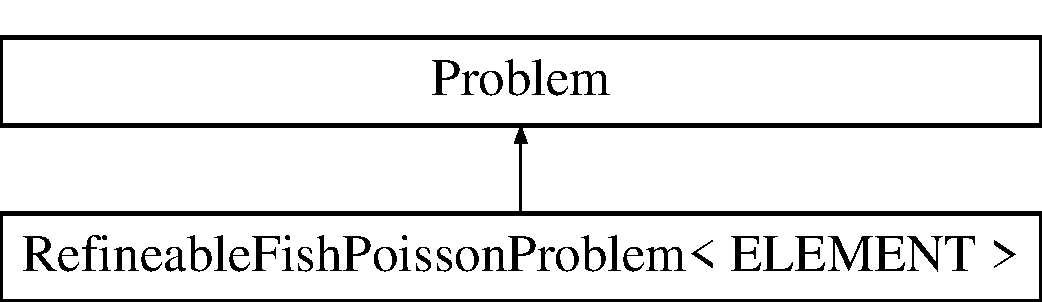
\includegraphics[height=2.000000cm]{classRefineableFishPoissonProblem}
\end{center}
\end{figure}
\subsection*{Public Member Functions}
\begin{DoxyCompactItemize}
\item 
\hyperlink{classRefineableFishPoissonProblem_a2585d906fab348e09bfb9b4c111ac161}{Refineable\+Fish\+Poisson\+Problem} (const bool \&fix\+\_\+position, const string \&directory\+\_\+name, const unsigned \&i\+\_\+case)
\begin{DoxyCompactList}\small\item\em Constructor\+: Bool flag specifies if position of fish back is prescribed or computed from the coupled problem. String specifies output directory. \end{DoxyCompactList}\item 
virtual \hyperlink{classRefineableFishPoissonProblem_a7039a3409520850908940927b91af9ab}{$\sim$\+Refineable\+Fish\+Poisson\+Problem} ()
\begin{DoxyCompactList}\small\item\em Destructor. \end{DoxyCompactList}\item 
void \hyperlink{classRefineableFishPoissonProblem_a8d8fb7ef1c571c57c02073edab4a7759}{actions\+\_\+before\+\_\+newton\+\_\+convergence\+\_\+check} ()
\begin{DoxyCompactList}\small\item\em Update after Newton step\+: Update mesh in response to possible changes in the wall shape. \end{DoxyCompactList}\item 
void \hyperlink{classRefineableFishPoissonProblem_a7f6c356f7c8bd0130de957297e999f40}{actions\+\_\+after\+\_\+newton\+\_\+solve} ()
\begin{DoxyCompactList}\small\item\em Update the problem specs after solve (empty) \end{DoxyCompactList}\item 
void \hyperlink{classRefineableFishPoissonProblem_a58098181f3b88c2fc65f24fb15c1a529}{actions\+\_\+before\+\_\+newton\+\_\+solve} ()
\begin{DoxyCompactList}\small\item\em Update the problem specs before solve\+: Update mesh. \end{DoxyCompactList}\item 
Algebraic\+Refineable\+Fish\+Mesh$<$ E\+L\+E\+M\+E\+NT $>$ $\ast$ \hyperlink{classRefineableFishPoissonProblem_a6f25d5110e5262e66e2900da051567a6}{fish\+\_\+mesh\+\_\+pt} ()
\item 
double \& \hyperlink{classRefineableFishPoissonProblem_a20702e8945d442c9597348b550da14e4}{load} ()
\begin{DoxyCompactList}\small\item\em Return value of the \char`\"{}load\char`\"{} on the elastically supported ring. \end{DoxyCompactList}\item 
double \& \hyperlink{classRefineableFishPoissonProblem_a152227cc825ddea07cb06c2791f5995b}{y\+\_\+c} ()
\begin{DoxyCompactList}\small\item\em Return value of the vertical displacement of the ring that represents the fish\textquotesingle{}s back. \end{DoxyCompactList}\item 
void \hyperlink{classRefineableFishPoissonProblem_a6db25ff0bd3014aa531d9f0e8b385beb}{doc\+\_\+solution} ()
\begin{DoxyCompactList}\small\item\em Doc the solution. \end{DoxyCompactList}\item 
Doc\+Info \& \hyperlink{classRefineableFishPoissonProblem_a093f5963e63746843c33ca444a205333}{doc\+\_\+info} ()
\begin{DoxyCompactList}\small\item\em Access to Doc\+Info object. \end{DoxyCompactList}\item 
\hyperlink{classRefineableFishPoissonProblem_a0211667b09b7da71184de2524609701f}{Refineable\+Fish\+Poisson\+Problem} (bool fix\+\_\+position, string directory\+\_\+name)
\begin{DoxyCompactList}\small\item\em Constructor\+: Bool flag specifies if position of fish back is prescribed or computed from the coupled problem. String specifies output directory. \end{DoxyCompactList}\item 
virtual \hyperlink{classRefineableFishPoissonProblem_a4a5e7c5f264364211ad641353933c222}{$\sim$\+Refineable\+Fish\+Poisson\+Problem} ()
\begin{DoxyCompactList}\small\item\em Destructor. \end{DoxyCompactList}\item 
void \hyperlink{classRefineableFishPoissonProblem_a8d8fb7ef1c571c57c02073edab4a7759}{actions\+\_\+before\+\_\+newton\+\_\+convergence\+\_\+check} ()
\begin{DoxyCompactList}\small\item\em Update after Newton step\+: Update in response to possible changes in the wall shape. \end{DoxyCompactList}\item 
void \hyperlink{classRefineableFishPoissonProblem_a58098181f3b88c2fc65f24fb15c1a529}{actions\+\_\+before\+\_\+newton\+\_\+solve} ()
\begin{DoxyCompactList}\small\item\em Update the problem specs before solve\+: Update nodal positions. \end{DoxyCompactList}\item 
void \hyperlink{classRefineableFishPoissonProblem_a7f6c356f7c8bd0130de957297e999f40}{actions\+\_\+after\+\_\+newton\+\_\+solve} ()
\begin{DoxyCompactList}\small\item\em Update the problem specs after solve (empty) \end{DoxyCompactList}\item 
Macro\+Element\+Node\+Update\+Refineable\+Fish\+Mesh$<$ E\+L\+E\+M\+E\+NT $>$ $\ast$ \hyperlink{classRefineableFishPoissonProblem_ab472201df89d71930157fbc45b8eaa54}{fish\+\_\+mesh\+\_\+pt} ()
\item 
double \& \hyperlink{classRefineableFishPoissonProblem_a20702e8945d442c9597348b550da14e4}{load} ()
\begin{DoxyCompactList}\small\item\em Return value of the \char`\"{}load\char`\"{} on the elastically supported ring that represents the fish\textquotesingle{}s back. \end{DoxyCompactList}\item 
double \& \hyperlink{classRefineableFishPoissonProblem_a152227cc825ddea07cb06c2791f5995b}{y\+\_\+c} ()
\begin{DoxyCompactList}\small\item\em Return value of the vertical displacement of the ring that represents the fish\textquotesingle{}s back. \end{DoxyCompactList}\item 
void \hyperlink{classRefineableFishPoissonProblem_a6db25ff0bd3014aa531d9f0e8b385beb}{doc\+\_\+solution} ()
\begin{DoxyCompactList}\small\item\em Doc the solution. \end{DoxyCompactList}\item 
Doc\+Info \& \hyperlink{classRefineableFishPoissonProblem_a093f5963e63746843c33ca444a205333}{doc\+\_\+info} ()
\begin{DoxyCompactList}\small\item\em Access to Doc\+Info object. \end{DoxyCompactList}\end{DoxyCompactItemize}
\subsection*{Private Member Functions}
\begin{DoxyCompactItemize}
\item 
void \hyperlink{classRefineableFishPoissonProblem_a122cddf55249eaf0ee813818ff101fb4}{set\+\_\+shape\+\_\+deriv\+\_\+method} ()
\begin{DoxyCompactList}\small\item\em Helper fct to set method for evaluation of shape derivs. \end{DoxyCompactList}\end{DoxyCompactItemize}
\subsection*{Private Attributes}
\begin{DoxyCompactItemize}
\item 
Node $\ast$ \hyperlink{classRefineableFishPoissonProblem_a5dce47aa14fdbc33d8a865f4f4b1e1ea}{Doc\+\_\+node\+\_\+pt}
\begin{DoxyCompactList}\small\item\em Node at which the solution of the Poisson equation is documented. \end{DoxyCompactList}\item 
ofstream \hyperlink{classRefineableFishPoissonProblem_aa358e2b0fa91780bdca32ae4676717ff}{Trace\+\_\+file}
\begin{DoxyCompactList}\small\item\em Trace file. \end{DoxyCompactList}\item 
Algebraic\+Refineable\+Fish\+Mesh$<$ E\+L\+E\+M\+E\+NT $>$ $\ast$ \hyperlink{classRefineableFishPoissonProblem_af915f09b6e4ae2f4ded2ad1a25ed7f01}{Fish\+\_\+mesh\+\_\+pt}
\begin{DoxyCompactList}\small\item\em Pointer to fish mesh. \end{DoxyCompactList}\item 
Mesh $\ast$ \hyperlink{classRefineableFishPoissonProblem_ac0f6f58b393715961214d98e11dfad57}{Fish\+\_\+back\+\_\+mesh\+\_\+pt}
\item 
Data $\ast$ \hyperlink{classRefineableFishPoissonProblem_a9a9ce82a4308be486701578134d06210}{Load\+\_\+pt}
\begin{DoxyCompactList}\small\item\em Pointer to data item that stores the \char`\"{}load\char`\"{} on the fish back. \end{DoxyCompactList}\item 
bool \hyperlink{classRefineableFishPoissonProblem_a51c10ea7cbf4ab61fd953f011f72a1c4}{Fix\+\_\+position}
\begin{DoxyCompactList}\small\item\em Is the position of the fish back prescribed? \end{DoxyCompactList}\item 
Doc\+Info \hyperlink{classRefineableFishPoissonProblem_ad6d382f1d38425323627f34e0559b28f}{Doc\+\_\+info}
\begin{DoxyCompactList}\small\item\em Doc info object. \end{DoxyCompactList}\item 
unsigned \hyperlink{classRefineableFishPoissonProblem_af6f409d7fe711ad809d9e784d98ca036}{Case\+\_\+id}
\begin{DoxyCompactList}\small\item\em Case id. \end{DoxyCompactList}\item 
Macro\+Element\+Node\+Update\+Refineable\+Fish\+Mesh$<$ E\+L\+E\+M\+E\+NT $>$ $\ast$ \hyperlink{classRefineableFishPoissonProblem_a769ab4e05f6962a7c8fc85f03a261916}{Fish\+\_\+mesh\+\_\+pt}
\begin{DoxyCompactList}\small\item\em Pointer to fish mesh. \end{DoxyCompactList}\end{DoxyCompactItemize}


\subsection{Detailed Description}
\subsubsection*{template$<$class E\+L\+E\+M\+E\+NT$>$\newline
class Refineable\+Fish\+Poisson\+Problem$<$ E\+L\+E\+M\+E\+N\+T $>$}

Refineable Poisson problem in deformable fish-\/shaped domain. Template parameter identify the elements.

Refineable Poisson problem in deformable fish-\/shaped domain. Template parameter identifies the element. 

Definition at line 84 of file algebraic\+\_\+free\+\_\+boundary\+\_\+poisson.\+cc.



\subsection{Constructor \& Destructor Documentation}
\mbox{\Hypertarget{classRefineableFishPoissonProblem_a2585d906fab348e09bfb9b4c111ac161}\label{classRefineableFishPoissonProblem_a2585d906fab348e09bfb9b4c111ac161}} 
\index{Refineable\+Fish\+Poisson\+Problem@{Refineable\+Fish\+Poisson\+Problem}!Refineable\+Fish\+Poisson\+Problem@{Refineable\+Fish\+Poisson\+Problem}}
\index{Refineable\+Fish\+Poisson\+Problem@{Refineable\+Fish\+Poisson\+Problem}!Refineable\+Fish\+Poisson\+Problem@{Refineable\+Fish\+Poisson\+Problem}}
\subsubsection{\texorpdfstring{Refineable\+Fish\+Poisson\+Problem()}{RefineableFishPoissonProblem()}\hspace{0.1cm}{\footnotesize\ttfamily [1/2]}}
{\footnotesize\ttfamily template$<$class E\+L\+E\+M\+E\+NT $>$ \\
\hyperlink{classRefineableFishPoissonProblem}{Refineable\+Fish\+Poisson\+Problem}$<$ E\+L\+E\+M\+E\+NT $>$\+::\hyperlink{classRefineableFishPoissonProblem}{Refineable\+Fish\+Poisson\+Problem} (\begin{DoxyParamCaption}\item[{const bool \&}]{fix\+\_\+position,  }\item[{const string \&}]{directory\+\_\+name,  }\item[{const unsigned \&}]{i\+\_\+case }\end{DoxyParamCaption})}



Constructor\+: Bool flag specifies if position of fish back is prescribed or computed from the coupled problem. String specifies output directory. 

Constructor for adaptive Poisson problem in deformable fish-\/shaped domain. Pass flag if position of fish back is fixed, and the output directory. Loop over elements and set pointers to source function 

Definition at line 244 of file algebraic\+\_\+free\+\_\+boundary\+\_\+poisson.\+cc.



References Refineable\+Fish\+Poisson\+Problem$<$ E\+L\+E\+M\+E\+N\+T $>$\+::\+Doc\+\_\+info, Refineable\+Fish\+Poisson\+Problem$<$ E\+L\+E\+M\+E\+N\+T $>$\+::\+Doc\+\_\+node\+\_\+pt, Refineable\+Fish\+Poisson\+Problem$<$ E\+L\+E\+M\+E\+N\+T $>$\+::\+Fish\+\_\+back\+\_\+mesh\+\_\+pt, Refineable\+Fish\+Poisson\+Problem$<$ E\+L\+E\+M\+E\+N\+T $>$\+::fish\+\_\+mesh\+\_\+pt(), Refineable\+Fish\+Poisson\+Problem$<$ E\+L\+E\+M\+E\+N\+T $>$\+::\+Fish\+\_\+mesh\+\_\+pt, Refineable\+Fish\+Poisson\+Problem$<$ E\+L\+E\+M\+E\+N\+T $>$\+::\+Fix\+\_\+position, Const\+Source\+For\+Poisson\+::get\+\_\+source(), Refineable\+Fish\+Poisson\+Problem$<$ E\+L\+E\+M\+E\+N\+T $>$\+::\+Load\+\_\+pt, Refineable\+Fish\+Poisson\+Problem$<$ E\+L\+E\+M\+E\+N\+T $>$\+::set\+\_\+shape\+\_\+deriv\+\_\+method(), Refineable\+Fish\+Poisson\+Problem$<$ E\+L\+E\+M\+E\+N\+T $>$\+::\+Trace\+\_\+file, and Refineable\+Fish\+Poisson\+Problem$<$ E\+L\+E\+M\+E\+N\+T $>$\+::y\+\_\+c().

\mbox{\Hypertarget{classRefineableFishPoissonProblem_a7039a3409520850908940927b91af9ab}\label{classRefineableFishPoissonProblem_a7039a3409520850908940927b91af9ab}} 
\index{Refineable\+Fish\+Poisson\+Problem@{Refineable\+Fish\+Poisson\+Problem}!````~Refineable\+Fish\+Poisson\+Problem@{$\sim$\+Refineable\+Fish\+Poisson\+Problem}}
\index{````~Refineable\+Fish\+Poisson\+Problem@{$\sim$\+Refineable\+Fish\+Poisson\+Problem}!Refineable\+Fish\+Poisson\+Problem@{Refineable\+Fish\+Poisson\+Problem}}
\subsubsection{\texorpdfstring{$\sim$\+Refineable\+Fish\+Poisson\+Problem()}{~RefineableFishPoissonProblem()}\hspace{0.1cm}{\footnotesize\ttfamily [1/2]}}
{\footnotesize\ttfamily template$<$class E\+L\+E\+M\+E\+NT $>$ \\
\hyperlink{classRefineableFishPoissonProblem}{Refineable\+Fish\+Poisson\+Problem}$<$ E\+L\+E\+M\+E\+NT $>$\+::$\sim$\hyperlink{classRefineableFishPoissonProblem}{Refineable\+Fish\+Poisson\+Problem} (\begin{DoxyParamCaption}{ }\end{DoxyParamCaption})\hspace{0.3cm}{\ttfamily [virtual]}}



Destructor. 

Destructor for Poisson problem in deformable fish-\/shaped domain. 

Definition at line 394 of file algebraic\+\_\+free\+\_\+boundary\+\_\+poisson.\+cc.



References Refineable\+Fish\+Poisson\+Problem$<$ E\+L\+E\+M\+E\+N\+T $>$\+::\+Trace\+\_\+file.



Referenced by Refineable\+Fish\+Poisson\+Problem$<$ E\+L\+E\+M\+E\+N\+T $>$\+::\+Refineable\+Fish\+Poisson\+Problem().

\mbox{\Hypertarget{classRefineableFishPoissonProblem_a0211667b09b7da71184de2524609701f}\label{classRefineableFishPoissonProblem_a0211667b09b7da71184de2524609701f}} 
\index{Refineable\+Fish\+Poisson\+Problem@{Refineable\+Fish\+Poisson\+Problem}!Refineable\+Fish\+Poisson\+Problem@{Refineable\+Fish\+Poisson\+Problem}}
\index{Refineable\+Fish\+Poisson\+Problem@{Refineable\+Fish\+Poisson\+Problem}!Refineable\+Fish\+Poisson\+Problem@{Refineable\+Fish\+Poisson\+Problem}}
\subsubsection{\texorpdfstring{Refineable\+Fish\+Poisson\+Problem()}{RefineableFishPoissonProblem()}\hspace{0.1cm}{\footnotesize\ttfamily [2/2]}}
{\footnotesize\ttfamily template$<$class E\+L\+E\+M\+E\+NT $>$ \\
\hyperlink{classRefineableFishPoissonProblem}{Refineable\+Fish\+Poisson\+Problem}$<$ E\+L\+E\+M\+E\+NT $>$\+::\hyperlink{classRefineableFishPoissonProblem}{Refineable\+Fish\+Poisson\+Problem} (\begin{DoxyParamCaption}\item[{bool}]{fix\+\_\+position,  }\item[{string}]{directory\+\_\+name }\end{DoxyParamCaption})}



Constructor\+: Bool flag specifies if position of fish back is prescribed or computed from the coupled problem. String specifies output directory. 

Constructor for adaptive Poisson problem in deformable fish-\/shaped domain. Pass flag if position of fish back is fixed, and the output directory. Loop over elements and set pointers to source function 

Definition at line 184 of file old\+\_\+for\+\_\+doc.\+cc.



References Refineable\+Fish\+Poisson\+Problem$<$ E\+L\+E\+M\+E\+N\+T $>$\+::\+Doc\+\_\+info, Refineable\+Fish\+Poisson\+Problem$<$ E\+L\+E\+M\+E\+N\+T $>$\+::\+Doc\+\_\+node\+\_\+pt, Refineable\+Fish\+Poisson\+Problem$<$ E\+L\+E\+M\+E\+N\+T $>$\+::doc\+\_\+solution(), Refineable\+Fish\+Poisson\+Problem$<$ E\+L\+E\+M\+E\+N\+T $>$\+::\+Fish\+\_\+back\+\_\+mesh\+\_\+pt, Refineable\+Fish\+Poisson\+Problem$<$ E\+L\+E\+M\+E\+N\+T $>$\+::fish\+\_\+mesh\+\_\+pt(), Refineable\+Fish\+Poisson\+Problem$<$ E\+L\+E\+M\+E\+N\+T $>$\+::\+Fish\+\_\+mesh\+\_\+pt, Refineable\+Fish\+Poisson\+Problem$<$ E\+L\+E\+M\+E\+N\+T $>$\+::\+Fix\+\_\+position, Const\+Source\+For\+Poisson\+::get\+\_\+source(), Refineable\+Fish\+Poisson\+Problem$<$ E\+L\+E\+M\+E\+N\+T $>$\+::load(), Refineable\+Fish\+Poisson\+Problem$<$ E\+L\+E\+M\+E\+N\+T $>$\+::\+Load\+\_\+pt, Refineable\+Fish\+Poisson\+Problem$<$ E\+L\+E\+M\+E\+N\+T $>$\+::\+Trace\+\_\+file, Refineable\+Fish\+Poisson\+Problem$<$ E\+L\+E\+M\+E\+N\+T $>$\+::y\+\_\+c(), and Refineable\+Fish\+Poisson\+Problem$<$ E\+L\+E\+M\+E\+N\+T $>$\+::$\sim$\+Refineable\+Fish\+Poisson\+Problem().

\mbox{\Hypertarget{classRefineableFishPoissonProblem_a4a5e7c5f264364211ad641353933c222}\label{classRefineableFishPoissonProblem_a4a5e7c5f264364211ad641353933c222}} 
\index{Refineable\+Fish\+Poisson\+Problem@{Refineable\+Fish\+Poisson\+Problem}!````~Refineable\+Fish\+Poisson\+Problem@{$\sim$\+Refineable\+Fish\+Poisson\+Problem}}
\index{````~Refineable\+Fish\+Poisson\+Problem@{$\sim$\+Refineable\+Fish\+Poisson\+Problem}!Refineable\+Fish\+Poisson\+Problem@{Refineable\+Fish\+Poisson\+Problem}}
\subsubsection{\texorpdfstring{$\sim$\+Refineable\+Fish\+Poisson\+Problem()}{~RefineableFishPoissonProblem()}\hspace{0.1cm}{\footnotesize\ttfamily [2/2]}}
{\footnotesize\ttfamily template$<$class E\+L\+E\+M\+E\+NT$>$ \\
virtual \hyperlink{classRefineableFishPoissonProblem}{Refineable\+Fish\+Poisson\+Problem}$<$ E\+L\+E\+M\+E\+NT $>$\+::$\sim$\hyperlink{classRefineableFishPoissonProblem}{Refineable\+Fish\+Poisson\+Problem} (\begin{DoxyParamCaption}{ }\end{DoxyParamCaption})\hspace{0.3cm}{\ttfamily [virtual]}}



Destructor. 



\subsection{Member Function Documentation}
\mbox{\Hypertarget{classRefineableFishPoissonProblem_a7f6c356f7c8bd0130de957297e999f40}\label{classRefineableFishPoissonProblem_a7f6c356f7c8bd0130de957297e999f40}} 
\index{Refineable\+Fish\+Poisson\+Problem@{Refineable\+Fish\+Poisson\+Problem}!actions\+\_\+after\+\_\+newton\+\_\+solve@{actions\+\_\+after\+\_\+newton\+\_\+solve}}
\index{actions\+\_\+after\+\_\+newton\+\_\+solve@{actions\+\_\+after\+\_\+newton\+\_\+solve}!Refineable\+Fish\+Poisson\+Problem@{Refineable\+Fish\+Poisson\+Problem}}
\subsubsection{\texorpdfstring{actions\+\_\+after\+\_\+newton\+\_\+solve()}{actions\_after\_newton\_solve()}\hspace{0.1cm}{\footnotesize\ttfamily [1/2]}}
{\footnotesize\ttfamily template$<$class E\+L\+E\+M\+E\+NT$>$ \\
void \hyperlink{classRefineableFishPoissonProblem}{Refineable\+Fish\+Poisson\+Problem}$<$ E\+L\+E\+M\+E\+NT $>$\+::actions\+\_\+after\+\_\+newton\+\_\+solve (\begin{DoxyParamCaption}{ }\end{DoxyParamCaption})\hspace{0.3cm}{\ttfamily [inline]}}



Update the problem specs after solve (empty) 



Definition at line 107 of file algebraic\+\_\+free\+\_\+boundary\+\_\+poisson.\+cc.

\mbox{\Hypertarget{classRefineableFishPoissonProblem_a7f6c356f7c8bd0130de957297e999f40}\label{classRefineableFishPoissonProblem_a7f6c356f7c8bd0130de957297e999f40}} 
\index{Refineable\+Fish\+Poisson\+Problem@{Refineable\+Fish\+Poisson\+Problem}!actions\+\_\+after\+\_\+newton\+\_\+solve@{actions\+\_\+after\+\_\+newton\+\_\+solve}}
\index{actions\+\_\+after\+\_\+newton\+\_\+solve@{actions\+\_\+after\+\_\+newton\+\_\+solve}!Refineable\+Fish\+Poisson\+Problem@{Refineable\+Fish\+Poisson\+Problem}}
\subsubsection{\texorpdfstring{actions\+\_\+after\+\_\+newton\+\_\+solve()}{actions\_after\_newton\_solve()}\hspace{0.1cm}{\footnotesize\ttfamily [2/2]}}
{\footnotesize\ttfamily template$<$class E\+L\+E\+M\+E\+NT$>$ \\
void \hyperlink{classRefineableFishPoissonProblem}{Refineable\+Fish\+Poisson\+Problem}$<$ E\+L\+E\+M\+E\+NT $>$\+::actions\+\_\+after\+\_\+newton\+\_\+solve (\begin{DoxyParamCaption}{ }\end{DoxyParamCaption})\hspace{0.3cm}{\ttfamily [inline]}}



Update the problem specs after solve (empty) 



Definition at line 117 of file old\+\_\+for\+\_\+doc.\+cc.

\mbox{\Hypertarget{classRefineableFishPoissonProblem_a8d8fb7ef1c571c57c02073edab4a7759}\label{classRefineableFishPoissonProblem_a8d8fb7ef1c571c57c02073edab4a7759}} 
\index{Refineable\+Fish\+Poisson\+Problem@{Refineable\+Fish\+Poisson\+Problem}!actions\+\_\+before\+\_\+newton\+\_\+convergence\+\_\+check@{actions\+\_\+before\+\_\+newton\+\_\+convergence\+\_\+check}}
\index{actions\+\_\+before\+\_\+newton\+\_\+convergence\+\_\+check@{actions\+\_\+before\+\_\+newton\+\_\+convergence\+\_\+check}!Refineable\+Fish\+Poisson\+Problem@{Refineable\+Fish\+Poisson\+Problem}}
\subsubsection{\texorpdfstring{actions\+\_\+before\+\_\+newton\+\_\+convergence\+\_\+check()}{actions\_before\_newton\_convergence\_check()}\hspace{0.1cm}{\footnotesize\ttfamily [1/2]}}
{\footnotesize\ttfamily template$<$class E\+L\+E\+M\+E\+NT$>$ \\
void \hyperlink{classRefineableFishPoissonProblem}{Refineable\+Fish\+Poisson\+Problem}$<$ E\+L\+E\+M\+E\+NT $>$\+::actions\+\_\+before\+\_\+newton\+\_\+convergence\+\_\+check (\begin{DoxyParamCaption}{ }\end{DoxyParamCaption})\hspace{0.3cm}{\ttfamily [inline]}}



Update after Newton step\+: Update mesh in response to possible changes in the wall shape. 



Definition at line 101 of file algebraic\+\_\+free\+\_\+boundary\+\_\+poisson.\+cc.

\mbox{\Hypertarget{classRefineableFishPoissonProblem_a8d8fb7ef1c571c57c02073edab4a7759}\label{classRefineableFishPoissonProblem_a8d8fb7ef1c571c57c02073edab4a7759}} 
\index{Refineable\+Fish\+Poisson\+Problem@{Refineable\+Fish\+Poisson\+Problem}!actions\+\_\+before\+\_\+newton\+\_\+convergence\+\_\+check@{actions\+\_\+before\+\_\+newton\+\_\+convergence\+\_\+check}}
\index{actions\+\_\+before\+\_\+newton\+\_\+convergence\+\_\+check@{actions\+\_\+before\+\_\+newton\+\_\+convergence\+\_\+check}!Refineable\+Fish\+Poisson\+Problem@{Refineable\+Fish\+Poisson\+Problem}}
\subsubsection{\texorpdfstring{actions\+\_\+before\+\_\+newton\+\_\+convergence\+\_\+check()}{actions\_before\_newton\_convergence\_check()}\hspace{0.1cm}{\footnotesize\ttfamily [2/2]}}
{\footnotesize\ttfamily template$<$class E\+L\+E\+M\+E\+NT$>$ \\
void \hyperlink{classRefineableFishPoissonProblem}{Refineable\+Fish\+Poisson\+Problem}$<$ E\+L\+E\+M\+E\+NT $>$\+::actions\+\_\+before\+\_\+newton\+\_\+convergence\+\_\+check (\begin{DoxyParamCaption}{ }\end{DoxyParamCaption})\hspace{0.3cm}{\ttfamily [inline]}}



Update after Newton step\+: Update in response to possible changes in the wall shape. 



Definition at line 104 of file old\+\_\+for\+\_\+doc.\+cc.

\mbox{\Hypertarget{classRefineableFishPoissonProblem_a58098181f3b88c2fc65f24fb15c1a529}\label{classRefineableFishPoissonProblem_a58098181f3b88c2fc65f24fb15c1a529}} 
\index{Refineable\+Fish\+Poisson\+Problem@{Refineable\+Fish\+Poisson\+Problem}!actions\+\_\+before\+\_\+newton\+\_\+solve@{actions\+\_\+before\+\_\+newton\+\_\+solve}}
\index{actions\+\_\+before\+\_\+newton\+\_\+solve@{actions\+\_\+before\+\_\+newton\+\_\+solve}!Refineable\+Fish\+Poisson\+Problem@{Refineable\+Fish\+Poisson\+Problem}}
\subsubsection{\texorpdfstring{actions\+\_\+before\+\_\+newton\+\_\+solve()}{actions\_before\_newton\_solve()}\hspace{0.1cm}{\footnotesize\ttfamily [1/2]}}
{\footnotesize\ttfamily template$<$class E\+L\+E\+M\+E\+NT$>$ \\
void \hyperlink{classRefineableFishPoissonProblem}{Refineable\+Fish\+Poisson\+Problem}$<$ E\+L\+E\+M\+E\+NT $>$\+::actions\+\_\+before\+\_\+newton\+\_\+solve (\begin{DoxyParamCaption}{ }\end{DoxyParamCaption})\hspace{0.3cm}{\ttfamily [inline]}}



Update the problem specs before solve\+: Update mesh. 



Definition at line 110 of file algebraic\+\_\+free\+\_\+boundary\+\_\+poisson.\+cc.

\mbox{\Hypertarget{classRefineableFishPoissonProblem_a58098181f3b88c2fc65f24fb15c1a529}\label{classRefineableFishPoissonProblem_a58098181f3b88c2fc65f24fb15c1a529}} 
\index{Refineable\+Fish\+Poisson\+Problem@{Refineable\+Fish\+Poisson\+Problem}!actions\+\_\+before\+\_\+newton\+\_\+solve@{actions\+\_\+before\+\_\+newton\+\_\+solve}}
\index{actions\+\_\+before\+\_\+newton\+\_\+solve@{actions\+\_\+before\+\_\+newton\+\_\+solve}!Refineable\+Fish\+Poisson\+Problem@{Refineable\+Fish\+Poisson\+Problem}}
\subsubsection{\texorpdfstring{actions\+\_\+before\+\_\+newton\+\_\+solve()}{actions\_before\_newton\_solve()}\hspace{0.1cm}{\footnotesize\ttfamily [2/2]}}
{\footnotesize\ttfamily template$<$class E\+L\+E\+M\+E\+NT$>$ \\
void \hyperlink{classRefineableFishPoissonProblem}{Refineable\+Fish\+Poisson\+Problem}$<$ E\+L\+E\+M\+E\+NT $>$\+::actions\+\_\+before\+\_\+newton\+\_\+solve (\begin{DoxyParamCaption}{ }\end{DoxyParamCaption})\hspace{0.3cm}{\ttfamily [inline]}}



Update the problem specs before solve\+: Update nodal positions. 



Definition at line 111 of file old\+\_\+for\+\_\+doc.\+cc.

\mbox{\Hypertarget{classRefineableFishPoissonProblem_a093f5963e63746843c33ca444a205333}\label{classRefineableFishPoissonProblem_a093f5963e63746843c33ca444a205333}} 
\index{Refineable\+Fish\+Poisson\+Problem@{Refineable\+Fish\+Poisson\+Problem}!doc\+\_\+info@{doc\+\_\+info}}
\index{doc\+\_\+info@{doc\+\_\+info}!Refineable\+Fish\+Poisson\+Problem@{Refineable\+Fish\+Poisson\+Problem}}
\subsubsection{\texorpdfstring{doc\+\_\+info()}{doc\_info()}\hspace{0.1cm}{\footnotesize\ttfamily [1/2]}}
{\footnotesize\ttfamily template$<$class E\+L\+E\+M\+E\+NT$>$ \\
Doc\+Info\& \hyperlink{classRefineableFishPoissonProblem}{Refineable\+Fish\+Poisson\+Problem}$<$ E\+L\+E\+M\+E\+NT $>$\+::doc\+\_\+info (\begin{DoxyParamCaption}{ }\end{DoxyParamCaption})\hspace{0.3cm}{\ttfamily [inline]}}



Access to Doc\+Info object. 



Definition at line 140 of file algebraic\+\_\+free\+\_\+boundary\+\_\+poisson.\+cc.



Referenced by demo\+\_\+fish\+\_\+poisson().

\mbox{\Hypertarget{classRefineableFishPoissonProblem_a093f5963e63746843c33ca444a205333}\label{classRefineableFishPoissonProblem_a093f5963e63746843c33ca444a205333}} 
\index{Refineable\+Fish\+Poisson\+Problem@{Refineable\+Fish\+Poisson\+Problem}!doc\+\_\+info@{doc\+\_\+info}}
\index{doc\+\_\+info@{doc\+\_\+info}!Refineable\+Fish\+Poisson\+Problem@{Refineable\+Fish\+Poisson\+Problem}}
\subsubsection{\texorpdfstring{doc\+\_\+info()}{doc\_info()}\hspace{0.1cm}{\footnotesize\ttfamily [2/2]}}
{\footnotesize\ttfamily template$<$class E\+L\+E\+M\+E\+NT$>$ \\
Doc\+Info\& \hyperlink{classRefineableFishPoissonProblem}{Refineable\+Fish\+Poisson\+Problem}$<$ E\+L\+E\+M\+E\+NT $>$\+::doc\+\_\+info (\begin{DoxyParamCaption}{ }\end{DoxyParamCaption})\hspace{0.3cm}{\ttfamily [inline]}}



Access to Doc\+Info object. 



Definition at line 144 of file old\+\_\+for\+\_\+doc.\+cc.

\mbox{\Hypertarget{classRefineableFishPoissonProblem_a6db25ff0bd3014aa531d9f0e8b385beb}\label{classRefineableFishPoissonProblem_a6db25ff0bd3014aa531d9f0e8b385beb}} 
\index{Refineable\+Fish\+Poisson\+Problem@{Refineable\+Fish\+Poisson\+Problem}!doc\+\_\+solution@{doc\+\_\+solution}}
\index{doc\+\_\+solution@{doc\+\_\+solution}!Refineable\+Fish\+Poisson\+Problem@{Refineable\+Fish\+Poisson\+Problem}}
\subsubsection{\texorpdfstring{doc\+\_\+solution()}{doc\_solution()}\hspace{0.1cm}{\footnotesize\ttfamily [1/2]}}
{\footnotesize\ttfamily template$<$class E\+L\+E\+M\+E\+NT $>$ \\
void \hyperlink{classRefineableFishPoissonProblem}{Refineable\+Fish\+Poisson\+Problem}$<$ E\+L\+E\+M\+E\+NT $>$\+::doc\+\_\+solution (\begin{DoxyParamCaption}{ }\end{DoxyParamCaption})}



Doc the solution. 

Doc the solution in tecplot format. 

Definition at line 408 of file algebraic\+\_\+free\+\_\+boundary\+\_\+poisson.\+cc.



References Refineable\+Fish\+Poisson\+Problem$<$ E\+L\+E\+M\+E\+N\+T $>$\+::\+Case\+\_\+id, Refineable\+Fish\+Poisson\+Problem$<$ E\+L\+E\+M\+E\+N\+T $>$\+::\+Doc\+\_\+info, Refineable\+Fish\+Poisson\+Problem$<$ E\+L\+E\+M\+E\+N\+T $>$\+::\+Doc\+\_\+node\+\_\+pt, Refineable\+Fish\+Poisson\+Problem$<$ E\+L\+E\+M\+E\+N\+T $>$\+::fish\+\_\+mesh\+\_\+pt(), Refineable\+Fish\+Poisson\+Problem$<$ E\+L\+E\+M\+E\+N\+T $>$\+::load(), Refineable\+Fish\+Poisson\+Problem$<$ E\+L\+E\+M\+E\+N\+T $>$\+::\+Trace\+\_\+file, and Refineable\+Fish\+Poisson\+Problem$<$ E\+L\+E\+M\+E\+N\+T $>$\+::y\+\_\+c().



Referenced by demo\+\_\+elastic\+\_\+fish\+\_\+poisson(), demo\+\_\+fish\+\_\+poisson(), and Refineable\+Fish\+Poisson\+Problem$<$ E\+L\+E\+M\+E\+N\+T $>$\+::\+Refineable\+Fish\+Poisson\+Problem().

\mbox{\Hypertarget{classRefineableFishPoissonProblem_a6db25ff0bd3014aa531d9f0e8b385beb}\label{classRefineableFishPoissonProblem_a6db25ff0bd3014aa531d9f0e8b385beb}} 
\index{Refineable\+Fish\+Poisson\+Problem@{Refineable\+Fish\+Poisson\+Problem}!doc\+\_\+solution@{doc\+\_\+solution}}
\index{doc\+\_\+solution@{doc\+\_\+solution}!Refineable\+Fish\+Poisson\+Problem@{Refineable\+Fish\+Poisson\+Problem}}
\subsubsection{\texorpdfstring{doc\+\_\+solution()}{doc\_solution()}\hspace{0.1cm}{\footnotesize\ttfamily [2/2]}}
{\footnotesize\ttfamily template$<$class E\+L\+E\+M\+E\+NT$>$ \\
void \hyperlink{classRefineableFishPoissonProblem}{Refineable\+Fish\+Poisson\+Problem}$<$ E\+L\+E\+M\+E\+NT $>$\+::doc\+\_\+solution (\begin{DoxyParamCaption}{ }\end{DoxyParamCaption})}



Doc the solution. 

\mbox{\Hypertarget{classRefineableFishPoissonProblem_a6f25d5110e5262e66e2900da051567a6}\label{classRefineableFishPoissonProblem_a6f25d5110e5262e66e2900da051567a6}} 
\index{Refineable\+Fish\+Poisson\+Problem@{Refineable\+Fish\+Poisson\+Problem}!fish\+\_\+mesh\+\_\+pt@{fish\+\_\+mesh\+\_\+pt}}
\index{fish\+\_\+mesh\+\_\+pt@{fish\+\_\+mesh\+\_\+pt}!Refineable\+Fish\+Poisson\+Problem@{Refineable\+Fish\+Poisson\+Problem}}
\subsubsection{\texorpdfstring{fish\+\_\+mesh\+\_\+pt()}{fish\_mesh\_pt()}\hspace{0.1cm}{\footnotesize\ttfamily [1/2]}}
{\footnotesize\ttfamily template$<$class E\+L\+E\+M\+E\+NT$>$ \\
Algebraic\+Refineable\+Fish\+Mesh$<$E\+L\+E\+M\+E\+NT$>$$\ast$ \hyperlink{classRefineableFishPoissonProblem}{Refineable\+Fish\+Poisson\+Problem}$<$ E\+L\+E\+M\+E\+NT $>$\+::fish\+\_\+mesh\+\_\+pt (\begin{DoxyParamCaption}{ }\end{DoxyParamCaption})\hspace{0.3cm}{\ttfamily [inline]}}



Definition at line 116 of file algebraic\+\_\+free\+\_\+boundary\+\_\+poisson.\+cc.



Referenced by demo\+\_\+elastic\+\_\+fish\+\_\+poisson(), demo\+\_\+fish\+\_\+poisson(), Refineable\+Fish\+Poisson\+Problem$<$ E\+L\+E\+M\+E\+N\+T $>$\+::doc\+\_\+solution(), and Refineable\+Fish\+Poisson\+Problem$<$ E\+L\+E\+M\+E\+N\+T $>$\+::\+Refineable\+Fish\+Poisson\+Problem().

\mbox{\Hypertarget{classRefineableFishPoissonProblem_ab472201df89d71930157fbc45b8eaa54}\label{classRefineableFishPoissonProblem_ab472201df89d71930157fbc45b8eaa54}} 
\index{Refineable\+Fish\+Poisson\+Problem@{Refineable\+Fish\+Poisson\+Problem}!fish\+\_\+mesh\+\_\+pt@{fish\+\_\+mesh\+\_\+pt}}
\index{fish\+\_\+mesh\+\_\+pt@{fish\+\_\+mesh\+\_\+pt}!Refineable\+Fish\+Poisson\+Problem@{Refineable\+Fish\+Poisson\+Problem}}
\subsubsection{\texorpdfstring{fish\+\_\+mesh\+\_\+pt()}{fish\_mesh\_pt()}\hspace{0.1cm}{\footnotesize\ttfamily [2/2]}}
{\footnotesize\ttfamily template$<$class E\+L\+E\+M\+E\+NT$>$ \\
Macro\+Element\+Node\+Update\+Refineable\+Fish\+Mesh$<$E\+L\+E\+M\+E\+NT$>$$\ast$ \hyperlink{classRefineableFishPoissonProblem}{Refineable\+Fish\+Poisson\+Problem}$<$ E\+L\+E\+M\+E\+NT $>$\+::fish\+\_\+mesh\+\_\+pt (\begin{DoxyParamCaption}{ }\end{DoxyParamCaption})\hspace{0.3cm}{\ttfamily [inline]}}



Definition at line 120 of file old\+\_\+for\+\_\+doc.\+cc.

\mbox{\Hypertarget{classRefineableFishPoissonProblem_a20702e8945d442c9597348b550da14e4}\label{classRefineableFishPoissonProblem_a20702e8945d442c9597348b550da14e4}} 
\index{Refineable\+Fish\+Poisson\+Problem@{Refineable\+Fish\+Poisson\+Problem}!load@{load}}
\index{load@{load}!Refineable\+Fish\+Poisson\+Problem@{Refineable\+Fish\+Poisson\+Problem}}
\subsubsection{\texorpdfstring{load()}{load()}\hspace{0.1cm}{\footnotesize\ttfamily [1/2]}}
{\footnotesize\ttfamily template$<$class E\+L\+E\+M\+E\+NT$>$ \\
double\& \hyperlink{classRefineableFishPoissonProblem}{Refineable\+Fish\+Poisson\+Problem}$<$ E\+L\+E\+M\+E\+NT $>$\+::load (\begin{DoxyParamCaption}{ }\end{DoxyParamCaption})\hspace{0.3cm}{\ttfamily [inline]}}



Return value of the \char`\"{}load\char`\"{} on the elastically supported ring. 



Definition at line 122 of file algebraic\+\_\+free\+\_\+boundary\+\_\+poisson.\+cc.



Referenced by demo\+\_\+elastic\+\_\+fish\+\_\+poisson(), Refineable\+Fish\+Poisson\+Problem$<$ E\+L\+E\+M\+E\+N\+T $>$\+::doc\+\_\+solution(), and Refineable\+Fish\+Poisson\+Problem$<$ E\+L\+E\+M\+E\+N\+T $>$\+::\+Refineable\+Fish\+Poisson\+Problem().

\mbox{\Hypertarget{classRefineableFishPoissonProblem_a20702e8945d442c9597348b550da14e4}\label{classRefineableFishPoissonProblem_a20702e8945d442c9597348b550da14e4}} 
\index{Refineable\+Fish\+Poisson\+Problem@{Refineable\+Fish\+Poisson\+Problem}!load@{load}}
\index{load@{load}!Refineable\+Fish\+Poisson\+Problem@{Refineable\+Fish\+Poisson\+Problem}}
\subsubsection{\texorpdfstring{load()}{load()}\hspace{0.1cm}{\footnotesize\ttfamily [2/2]}}
{\footnotesize\ttfamily template$<$class E\+L\+E\+M\+E\+NT$>$ \\
double\& \hyperlink{classRefineableFishPoissonProblem}{Refineable\+Fish\+Poisson\+Problem}$<$ E\+L\+E\+M\+E\+NT $>$\+::load (\begin{DoxyParamCaption}{ }\end{DoxyParamCaption})\hspace{0.3cm}{\ttfamily [inline]}}



Return value of the \char`\"{}load\char`\"{} on the elastically supported ring that represents the fish\textquotesingle{}s back. 



Definition at line 127 of file old\+\_\+for\+\_\+doc.\+cc.

\mbox{\Hypertarget{classRefineableFishPoissonProblem_a122cddf55249eaf0ee813818ff101fb4}\label{classRefineableFishPoissonProblem_a122cddf55249eaf0ee813818ff101fb4}} 
\index{Refineable\+Fish\+Poisson\+Problem@{Refineable\+Fish\+Poisson\+Problem}!set\+\_\+shape\+\_\+deriv\+\_\+method@{set\+\_\+shape\+\_\+deriv\+\_\+method}}
\index{set\+\_\+shape\+\_\+deriv\+\_\+method@{set\+\_\+shape\+\_\+deriv\+\_\+method}!Refineable\+Fish\+Poisson\+Problem@{Refineable\+Fish\+Poisson\+Problem}}
\subsubsection{\texorpdfstring{set\+\_\+shape\+\_\+deriv\+\_\+method()}{set\_shape\_deriv\_method()}}
{\footnotesize\ttfamily template$<$class E\+L\+E\+M\+E\+NT$>$ \\
void \hyperlink{classRefineableFishPoissonProblem}{Refineable\+Fish\+Poisson\+Problem}$<$ E\+L\+E\+M\+E\+NT $>$\+::set\+\_\+shape\+\_\+deriv\+\_\+method (\begin{DoxyParamCaption}{ }\end{DoxyParamCaption})\hspace{0.3cm}{\ttfamily [inline]}, {\ttfamily [private]}}



Helper fct to set method for evaluation of shape derivs. 



Definition at line 145 of file algebraic\+\_\+free\+\_\+boundary\+\_\+poisson.\+cc.



Referenced by Refineable\+Fish\+Poisson\+Problem$<$ E\+L\+E\+M\+E\+N\+T $>$\+::\+Refineable\+Fish\+Poisson\+Problem().

\mbox{\Hypertarget{classRefineableFishPoissonProblem_a152227cc825ddea07cb06c2791f5995b}\label{classRefineableFishPoissonProblem_a152227cc825ddea07cb06c2791f5995b}} 
\index{Refineable\+Fish\+Poisson\+Problem@{Refineable\+Fish\+Poisson\+Problem}!y\+\_\+c@{y\+\_\+c}}
\index{y\+\_\+c@{y\+\_\+c}!Refineable\+Fish\+Poisson\+Problem@{Refineable\+Fish\+Poisson\+Problem}}
\subsubsection{\texorpdfstring{y\+\_\+c()}{y\_c()}\hspace{0.1cm}{\footnotesize\ttfamily [1/2]}}
{\footnotesize\ttfamily template$<$class E\+L\+E\+M\+E\+NT$>$ \\
double\& \hyperlink{classRefineableFishPoissonProblem}{Refineable\+Fish\+Poisson\+Problem}$<$ E\+L\+E\+M\+E\+NT $>$\+::y\+\_\+c (\begin{DoxyParamCaption}{ }\end{DoxyParamCaption})\hspace{0.3cm}{\ttfamily [inline]}}



Return value of the vertical displacement of the ring that represents the fish\textquotesingle{}s back. 



Definition at line 130 of file algebraic\+\_\+free\+\_\+boundary\+\_\+poisson.\+cc.



Referenced by demo\+\_\+fish\+\_\+poisson(), Refineable\+Fish\+Poisson\+Problem$<$ E\+L\+E\+M\+E\+N\+T $>$\+::doc\+\_\+solution(), and Refineable\+Fish\+Poisson\+Problem$<$ E\+L\+E\+M\+E\+N\+T $>$\+::\+Refineable\+Fish\+Poisson\+Problem().

\mbox{\Hypertarget{classRefineableFishPoissonProblem_a152227cc825ddea07cb06c2791f5995b}\label{classRefineableFishPoissonProblem_a152227cc825ddea07cb06c2791f5995b}} 
\index{Refineable\+Fish\+Poisson\+Problem@{Refineable\+Fish\+Poisson\+Problem}!y\+\_\+c@{y\+\_\+c}}
\index{y\+\_\+c@{y\+\_\+c}!Refineable\+Fish\+Poisson\+Problem@{Refineable\+Fish\+Poisson\+Problem}}
\subsubsection{\texorpdfstring{y\+\_\+c()}{y\_c()}\hspace{0.1cm}{\footnotesize\ttfamily [2/2]}}
{\footnotesize\ttfamily template$<$class E\+L\+E\+M\+E\+NT$>$ \\
double\& \hyperlink{classRefineableFishPoissonProblem}{Refineable\+Fish\+Poisson\+Problem}$<$ E\+L\+E\+M\+E\+NT $>$\+::y\+\_\+c (\begin{DoxyParamCaption}{ }\end{DoxyParamCaption})\hspace{0.3cm}{\ttfamily [inline]}}



Return value of the vertical displacement of the ring that represents the fish\textquotesingle{}s back. 



Definition at line 134 of file old\+\_\+for\+\_\+doc.\+cc.



\subsection{Member Data Documentation}
\mbox{\Hypertarget{classRefineableFishPoissonProblem_af6f409d7fe711ad809d9e784d98ca036}\label{classRefineableFishPoissonProblem_af6f409d7fe711ad809d9e784d98ca036}} 
\index{Refineable\+Fish\+Poisson\+Problem@{Refineable\+Fish\+Poisson\+Problem}!Case\+\_\+id@{Case\+\_\+id}}
\index{Case\+\_\+id@{Case\+\_\+id}!Refineable\+Fish\+Poisson\+Problem@{Refineable\+Fish\+Poisson\+Problem}}
\subsubsection{\texorpdfstring{Case\+\_\+id}{Case\_id}}
{\footnotesize\ttfamily template$<$class E\+L\+E\+M\+E\+NT$>$ \\
unsigned \hyperlink{classRefineableFishPoissonProblem}{Refineable\+Fish\+Poisson\+Problem}$<$ E\+L\+E\+M\+E\+NT $>$\+::Case\+\_\+id\hspace{0.3cm}{\ttfamily [private]}}



Case id. 



Definition at line 230 of file algebraic\+\_\+free\+\_\+boundary\+\_\+poisson.\+cc.



Referenced by Refineable\+Fish\+Poisson\+Problem$<$ E\+L\+E\+M\+E\+N\+T $>$\+::doc\+\_\+solution().

\mbox{\Hypertarget{classRefineableFishPoissonProblem_ad6d382f1d38425323627f34e0559b28f}\label{classRefineableFishPoissonProblem_ad6d382f1d38425323627f34e0559b28f}} 
\index{Refineable\+Fish\+Poisson\+Problem@{Refineable\+Fish\+Poisson\+Problem}!Doc\+\_\+info@{Doc\+\_\+info}}
\index{Doc\+\_\+info@{Doc\+\_\+info}!Refineable\+Fish\+Poisson\+Problem@{Refineable\+Fish\+Poisson\+Problem}}
\subsubsection{\texorpdfstring{Doc\+\_\+info}{Doc\_info}}
{\footnotesize\ttfamily template$<$class E\+L\+E\+M\+E\+NT$>$ \\
Doc\+Info \hyperlink{classRefineableFishPoissonProblem}{Refineable\+Fish\+Poisson\+Problem}$<$ E\+L\+E\+M\+E\+NT $>$\+::Doc\+\_\+info\hspace{0.3cm}{\ttfamily [private]}}



Doc info object. 



Definition at line 227 of file algebraic\+\_\+free\+\_\+boundary\+\_\+poisson.\+cc.



Referenced by Refineable\+Fish\+Poisson\+Problem$<$ E\+L\+E\+M\+E\+N\+T $>$\+::doc\+\_\+solution(), and Refineable\+Fish\+Poisson\+Problem$<$ E\+L\+E\+M\+E\+N\+T $>$\+::\+Refineable\+Fish\+Poisson\+Problem().

\mbox{\Hypertarget{classRefineableFishPoissonProblem_a5dce47aa14fdbc33d8a865f4f4b1e1ea}\label{classRefineableFishPoissonProblem_a5dce47aa14fdbc33d8a865f4f4b1e1ea}} 
\index{Refineable\+Fish\+Poisson\+Problem@{Refineable\+Fish\+Poisson\+Problem}!Doc\+\_\+node\+\_\+pt@{Doc\+\_\+node\+\_\+pt}}
\index{Doc\+\_\+node\+\_\+pt@{Doc\+\_\+node\+\_\+pt}!Refineable\+Fish\+Poisson\+Problem@{Refineable\+Fish\+Poisson\+Problem}}
\subsubsection{\texorpdfstring{Doc\+\_\+node\+\_\+pt}{Doc\_node\_pt}}
{\footnotesize\ttfamily template$<$class E\+L\+E\+M\+E\+NT$>$ \\
Node $\ast$ \hyperlink{classRefineableFishPoissonProblem}{Refineable\+Fish\+Poisson\+Problem}$<$ E\+L\+E\+M\+E\+NT $>$\+::Doc\+\_\+node\+\_\+pt\hspace{0.3cm}{\ttfamily [private]}}



Node at which the solution of the Poisson equation is documented. 

Node at which the solution of the Poisson equation is documented This solution at this node is also used as the \char`\"{}load\char`\"{} on the ring that represents the fish\textquotesingle{}s back. 

Definition at line 208 of file algebraic\+\_\+free\+\_\+boundary\+\_\+poisson.\+cc.



Referenced by Refineable\+Fish\+Poisson\+Problem$<$ E\+L\+E\+M\+E\+N\+T $>$\+::doc\+\_\+solution(), and Refineable\+Fish\+Poisson\+Problem$<$ E\+L\+E\+M\+E\+N\+T $>$\+::\+Refineable\+Fish\+Poisson\+Problem().

\mbox{\Hypertarget{classRefineableFishPoissonProblem_ac0f6f58b393715961214d98e11dfad57}\label{classRefineableFishPoissonProblem_ac0f6f58b393715961214d98e11dfad57}} 
\index{Refineable\+Fish\+Poisson\+Problem@{Refineable\+Fish\+Poisson\+Problem}!Fish\+\_\+back\+\_\+mesh\+\_\+pt@{Fish\+\_\+back\+\_\+mesh\+\_\+pt}}
\index{Fish\+\_\+back\+\_\+mesh\+\_\+pt@{Fish\+\_\+back\+\_\+mesh\+\_\+pt}!Refineable\+Fish\+Poisson\+Problem@{Refineable\+Fish\+Poisson\+Problem}}
\subsubsection{\texorpdfstring{Fish\+\_\+back\+\_\+mesh\+\_\+pt}{Fish\_back\_mesh\_pt}}
{\footnotesize\ttfamily template$<$class E\+L\+E\+M\+E\+NT$>$ \\
Mesh $\ast$ \hyperlink{classRefineableFishPoissonProblem}{Refineable\+Fish\+Poisson\+Problem}$<$ E\+L\+E\+M\+E\+NT $>$\+::Fish\+\_\+back\+\_\+mesh\+\_\+pt\hspace{0.3cm}{\ttfamily [private]}}

Pointer to single-\/element mesh that stores the Generalised\+Element that represents the fish back

Pointer to single-\/element mesh that stores the Generalised\+Element that represents the fish\textquotesingle{}s back 

Definition at line 218 of file algebraic\+\_\+free\+\_\+boundary\+\_\+poisson.\+cc.



Referenced by Refineable\+Fish\+Poisson\+Problem$<$ E\+L\+E\+M\+E\+N\+T $>$\+::\+Refineable\+Fish\+Poisson\+Problem().

\mbox{\Hypertarget{classRefineableFishPoissonProblem_a769ab4e05f6962a7c8fc85f03a261916}\label{classRefineableFishPoissonProblem_a769ab4e05f6962a7c8fc85f03a261916}} 
\index{Refineable\+Fish\+Poisson\+Problem@{Refineable\+Fish\+Poisson\+Problem}!Fish\+\_\+mesh\+\_\+pt@{Fish\+\_\+mesh\+\_\+pt}}
\index{Fish\+\_\+mesh\+\_\+pt@{Fish\+\_\+mesh\+\_\+pt}!Refineable\+Fish\+Poisson\+Problem@{Refineable\+Fish\+Poisson\+Problem}}
\subsubsection{\texorpdfstring{Fish\+\_\+mesh\+\_\+pt}{Fish\_mesh\_pt}\hspace{0.1cm}{\footnotesize\ttfamily [1/2]}}
{\footnotesize\ttfamily template$<$class E\+L\+E\+M\+E\+NT$>$ \\
Macro\+Element\+Node\+Update\+Refineable\+Fish\+Mesh$<$E\+L\+E\+M\+E\+NT$>$$\ast$ \hyperlink{classRefineableFishPoissonProblem}{Refineable\+Fish\+Poisson\+Problem}$<$ E\+L\+E\+M\+E\+NT $>$\+::Fish\+\_\+mesh\+\_\+pt\hspace{0.3cm}{\ttfamily [private]}}



Pointer to fish mesh. 



Definition at line 157 of file old\+\_\+for\+\_\+doc.\+cc.

\mbox{\Hypertarget{classRefineableFishPoissonProblem_af915f09b6e4ae2f4ded2ad1a25ed7f01}\label{classRefineableFishPoissonProblem_af915f09b6e4ae2f4ded2ad1a25ed7f01}} 
\index{Refineable\+Fish\+Poisson\+Problem@{Refineable\+Fish\+Poisson\+Problem}!Fish\+\_\+mesh\+\_\+pt@{Fish\+\_\+mesh\+\_\+pt}}
\index{Fish\+\_\+mesh\+\_\+pt@{Fish\+\_\+mesh\+\_\+pt}!Refineable\+Fish\+Poisson\+Problem@{Refineable\+Fish\+Poisson\+Problem}}
\subsubsection{\texorpdfstring{Fish\+\_\+mesh\+\_\+pt}{Fish\_mesh\_pt}\hspace{0.1cm}{\footnotesize\ttfamily [2/2]}}
{\footnotesize\ttfamily template$<$class E\+L\+E\+M\+E\+NT$>$ \\
Algebraic\+Refineable\+Fish\+Mesh$<$E\+L\+E\+M\+E\+NT$>$$\ast$ \hyperlink{classRefineableFishPoissonProblem}{Refineable\+Fish\+Poisson\+Problem}$<$ E\+L\+E\+M\+E\+NT $>$\+::Fish\+\_\+mesh\+\_\+pt\hspace{0.3cm}{\ttfamily [private]}}



Pointer to fish mesh. 



Definition at line 214 of file algebraic\+\_\+free\+\_\+boundary\+\_\+poisson.\+cc.



Referenced by Refineable\+Fish\+Poisson\+Problem$<$ E\+L\+E\+M\+E\+N\+T $>$\+::\+Refineable\+Fish\+Poisson\+Problem().

\mbox{\Hypertarget{classRefineableFishPoissonProblem_a51c10ea7cbf4ab61fd953f011f72a1c4}\label{classRefineableFishPoissonProblem_a51c10ea7cbf4ab61fd953f011f72a1c4}} 
\index{Refineable\+Fish\+Poisson\+Problem@{Refineable\+Fish\+Poisson\+Problem}!Fix\+\_\+position@{Fix\+\_\+position}}
\index{Fix\+\_\+position@{Fix\+\_\+position}!Refineable\+Fish\+Poisson\+Problem@{Refineable\+Fish\+Poisson\+Problem}}
\subsubsection{\texorpdfstring{Fix\+\_\+position}{Fix\_position}}
{\footnotesize\ttfamily template$<$class E\+L\+E\+M\+E\+NT$>$ \\
bool \hyperlink{classRefineableFishPoissonProblem}{Refineable\+Fish\+Poisson\+Problem}$<$ E\+L\+E\+M\+E\+NT $>$\+::Fix\+\_\+position\hspace{0.3cm}{\ttfamily [private]}}



Is the position of the fish back prescribed? 

Is the position of the fish\textquotesingle{}s back prescribed? 

Definition at line 224 of file algebraic\+\_\+free\+\_\+boundary\+\_\+poisson.\+cc.



Referenced by Refineable\+Fish\+Poisson\+Problem$<$ E\+L\+E\+M\+E\+N\+T $>$\+::\+Refineable\+Fish\+Poisson\+Problem().

\mbox{\Hypertarget{classRefineableFishPoissonProblem_a9a9ce82a4308be486701578134d06210}\label{classRefineableFishPoissonProblem_a9a9ce82a4308be486701578134d06210}} 
\index{Refineable\+Fish\+Poisson\+Problem@{Refineable\+Fish\+Poisson\+Problem}!Load\+\_\+pt@{Load\+\_\+pt}}
\index{Load\+\_\+pt@{Load\+\_\+pt}!Refineable\+Fish\+Poisson\+Problem@{Refineable\+Fish\+Poisson\+Problem}}
\subsubsection{\texorpdfstring{Load\+\_\+pt}{Load\_pt}}
{\footnotesize\ttfamily template$<$class E\+L\+E\+M\+E\+NT$>$ \\
Data $\ast$ \hyperlink{classRefineableFishPoissonProblem}{Refineable\+Fish\+Poisson\+Problem}$<$ E\+L\+E\+M\+E\+NT $>$\+::Load\+\_\+pt\hspace{0.3cm}{\ttfamily [private]}}



Pointer to data item that stores the \char`\"{}load\char`\"{} on the fish back. 



Definition at line 221 of file algebraic\+\_\+free\+\_\+boundary\+\_\+poisson.\+cc.



Referenced by Refineable\+Fish\+Poisson\+Problem$<$ E\+L\+E\+M\+E\+N\+T $>$\+::\+Refineable\+Fish\+Poisson\+Problem().

\mbox{\Hypertarget{classRefineableFishPoissonProblem_aa358e2b0fa91780bdca32ae4676717ff}\label{classRefineableFishPoissonProblem_aa358e2b0fa91780bdca32ae4676717ff}} 
\index{Refineable\+Fish\+Poisson\+Problem@{Refineable\+Fish\+Poisson\+Problem}!Trace\+\_\+file@{Trace\+\_\+file}}
\index{Trace\+\_\+file@{Trace\+\_\+file}!Refineable\+Fish\+Poisson\+Problem@{Refineable\+Fish\+Poisson\+Problem}}
\subsubsection{\texorpdfstring{Trace\+\_\+file}{Trace\_file}}
{\footnotesize\ttfamily template$<$class E\+L\+E\+M\+E\+NT$>$ \\
ofstream \hyperlink{classRefineableFishPoissonProblem}{Refineable\+Fish\+Poisson\+Problem}$<$ E\+L\+E\+M\+E\+NT $>$\+::Trace\+\_\+file\hspace{0.3cm}{\ttfamily [private]}}



Trace file. 



Definition at line 211 of file algebraic\+\_\+free\+\_\+boundary\+\_\+poisson.\+cc.



Referenced by Refineable\+Fish\+Poisson\+Problem$<$ E\+L\+E\+M\+E\+N\+T $>$\+::doc\+\_\+solution(), Refineable\+Fish\+Poisson\+Problem$<$ E\+L\+E\+M\+E\+N\+T $>$\+::\+Refineable\+Fish\+Poisson\+Problem(), and Refineable\+Fish\+Poisson\+Problem$<$ E\+L\+E\+M\+E\+N\+T $>$\+::$\sim$\+Refineable\+Fish\+Poisson\+Problem().



The documentation for this class was generated from the following files\+:\begin{DoxyCompactItemize}
\item 
\hyperlink{algebraic__free__boundary__poisson_8cc}{algebraic\+\_\+free\+\_\+boundary\+\_\+poisson.\+cc}\item 
\hyperlink{old__for__doc_8cc}{old\+\_\+for\+\_\+doc.\+cc}\end{DoxyCompactItemize}

\chapter{File Documentation}
\hypertarget{fish__poisson_8cc}{}\section{fish\+\_\+poisson.\+cc File Reference}
\label{fish__poisson_8cc}\index{fish\+\_\+poisson.\+cc@{fish\+\_\+poisson.\+cc}}
\subsection*{Classes}
\begin{DoxyCompactItemize}
\item 
class \hyperlink{classRefineableFishPoissonProblem}{Refineable\+Fish\+Poisson\+Problem$<$ E\+L\+E\+M\+E\+N\+T $>$}
\end{DoxyCompactItemize}
\subsection*{Namespaces}
\begin{DoxyCompactItemize}
\item 
 \hyperlink{namespaceConstSourceForPoisson}{Const\+Source\+For\+Poisson}
\begin{DoxyCompactList}\small\item\em Namespace for const source term in Poisson equation. \end{DoxyCompactList}\end{DoxyCompactItemize}
\subsection*{Functions}
\begin{DoxyCompactItemize}
\item 
void \hyperlink{namespaceConstSourceForPoisson_aeaa1153817bde9598372b803342f3299}{Const\+Source\+For\+Poisson\+::source\+\_\+function} (const Vector$<$ double $>$ \&x, double \&source)
\begin{DoxyCompactList}\small\item\em Const source function. \end{DoxyCompactList}\item 
void \hyperlink{fish__poisson_8cc_a9f5ae2c03a7f02e61857d322177ce5d5}{solve\+\_\+with\+\_\+incremental\+\_\+adaptation} ()
\item 
void \hyperlink{fish__poisson_8cc_a79a1cfcdcd821bd277276d163b85acfb}{solve\+\_\+with\+\_\+fully\+\_\+automatic\+\_\+adaptation} ()
\item 
int \hyperlink{fish__poisson_8cc_ae66f6b31b5ad750f1fe042a706a4e3d4}{main} ()
\end{DoxyCompactItemize}
\subsection*{Variables}
\begin{DoxyCompactItemize}
\item 
double \hyperlink{namespaceConstSourceForPoisson_add351c5acab2561d68d1fc9ec3d5fc5e}{Const\+Source\+For\+Poisson\+::\+Strength} =-\/1.\+0
\begin{DoxyCompactList}\small\item\em Strength of source function\+: default value -\/1.\+0. \end{DoxyCompactList}\end{DoxyCompactItemize}


\subsection{Function Documentation}
\mbox{\Hypertarget{fish__poisson_8cc_ae66f6b31b5ad750f1fe042a706a4e3d4}\label{fish__poisson_8cc_ae66f6b31b5ad750f1fe042a706a4e3d4}} 
\index{fish\+\_\+poisson.\+cc@{fish\+\_\+poisson.\+cc}!main@{main}}
\index{main@{main}!fish\+\_\+poisson.\+cc@{fish\+\_\+poisson.\+cc}}
\subsubsection{\texorpdfstring{main()}{main()}}
{\footnotesize\ttfamily int main (\begin{DoxyParamCaption}{ }\end{DoxyParamCaption})}

Demonstrate how to solve 2D Poisson problem in fish-\/shaped domain with mesh adaptation. 

Definition at line 329 of file fish\+\_\+poisson.\+cc.



References solve\+\_\+with\+\_\+fully\+\_\+automatic\+\_\+adaptation(), and solve\+\_\+with\+\_\+incremental\+\_\+adaptation().

\mbox{\Hypertarget{fish__poisson_8cc_a79a1cfcdcd821bd277276d163b85acfb}\label{fish__poisson_8cc_a79a1cfcdcd821bd277276d163b85acfb}} 
\index{fish\+\_\+poisson.\+cc@{fish\+\_\+poisson.\+cc}!solve\+\_\+with\+\_\+fully\+\_\+automatic\+\_\+adaptation@{solve\+\_\+with\+\_\+fully\+\_\+automatic\+\_\+adaptation}}
\index{solve\+\_\+with\+\_\+fully\+\_\+automatic\+\_\+adaptation@{solve\+\_\+with\+\_\+fully\+\_\+automatic\+\_\+adaptation}!fish\+\_\+poisson.\+cc@{fish\+\_\+poisson.\+cc}}
\subsubsection{\texorpdfstring{solve\+\_\+with\+\_\+fully\+\_\+automatic\+\_\+adaptation()}{solve\_with\_fully\_automatic\_adaptation()}}
{\footnotesize\ttfamily void solve\+\_\+with\+\_\+fully\+\_\+automatic\+\_\+adaptation (\begin{DoxyParamCaption}{ }\end{DoxyParamCaption})}

Demonstrate how to solve 2D Poisson problem in fish-\/shaped domain with fully automatic mesh adaptation 

Definition at line 286 of file fish\+\_\+poisson.\+cc.



References Refineable\+Fish\+Poisson\+Problem$<$ E\+L\+E\+M\+E\+N\+T $>$\+::doc\+\_\+solution(), and Refineable\+Fish\+Poisson\+Problem$<$ E\+L\+E\+M\+E\+N\+T $>$\+::mesh\+\_\+pt().



Referenced by main().

\mbox{\Hypertarget{fish__poisson_8cc_a9f5ae2c03a7f02e61857d322177ce5d5}\label{fish__poisson_8cc_a9f5ae2c03a7f02e61857d322177ce5d5}} 
\index{fish\+\_\+poisson.\+cc@{fish\+\_\+poisson.\+cc}!solve\+\_\+with\+\_\+incremental\+\_\+adaptation@{solve\+\_\+with\+\_\+incremental\+\_\+adaptation}}
\index{solve\+\_\+with\+\_\+incremental\+\_\+adaptation@{solve\+\_\+with\+\_\+incremental\+\_\+adaptation}!fish\+\_\+poisson.\+cc@{fish\+\_\+poisson.\+cc}}
\subsubsection{\texorpdfstring{solve\+\_\+with\+\_\+incremental\+\_\+adaptation()}{solve\_with\_incremental\_adaptation()}}
{\footnotesize\ttfamily void solve\+\_\+with\+\_\+incremental\+\_\+adaptation (\begin{DoxyParamCaption}{ }\end{DoxyParamCaption})}

Demonstrate how to solve 2D Poisson problem in fish-\/shaped domain with mesh adaptation. First we solve on the original coarse mesh. Next we do a few uniform refinement steps and re-\/solve. Finally, we enter into an automatic adapation loop. 

Definition at line 195 of file fish\+\_\+poisson.\+cc.



References Refineable\+Fish\+Poisson\+Problem$<$ E\+L\+E\+M\+E\+N\+T $>$\+::doc\+\_\+solution(), and Refineable\+Fish\+Poisson\+Problem$<$ E\+L\+E\+M\+E\+N\+T $>$\+::mesh\+\_\+pt().



Referenced by main().


\hypertarget{fish__poisson_8txt__doxygenified_8h}{}\section{fish\+\_\+poisson.\+txt\+\_\+doxygenified.\+h File Reference}
\label{fish__poisson_8txt__doxygenified_8h}\index{fish\+\_\+poisson.\+txt\+\_\+doxygenified.\+h@{fish\+\_\+poisson.\+txt\+\_\+doxygenified.\+h}}

\hypertarget{fish__poisson__no__adapt_8cc}{}\section{fish\+\_\+poisson\+\_\+no\+\_\+adapt.\+cc File Reference}
\label{fish__poisson__no__adapt_8cc}\index{fish\+\_\+poisson\+\_\+no\+\_\+adapt.\+cc@{fish\+\_\+poisson\+\_\+no\+\_\+adapt.\+cc}}
\subsection*{Classes}
\begin{DoxyCompactItemize}
\item 
class \hyperlink{classFishPoissonProblem}{Fish\+Poisson\+Problem$<$ E\+L\+E\+M\+E\+N\+T $>$}
\end{DoxyCompactItemize}
\subsection*{Namespaces}
\begin{DoxyCompactItemize}
\item 
 \hyperlink{namespaceConstSourceForPoisson}{Const\+Source\+For\+Poisson}
\begin{DoxyCompactList}\small\item\em Namespace for const source term in Poisson equation. \end{DoxyCompactList}\end{DoxyCompactItemize}
\subsection*{Functions}
\begin{DoxyCompactItemize}
\item 
void \hyperlink{namespaceConstSourceForPoisson_aeaa1153817bde9598372b803342f3299}{Const\+Source\+For\+Poisson\+::source\+\_\+function} (const Vector$<$ double $>$ \&x, double \&source)
\begin{DoxyCompactList}\small\item\em Const source function. \end{DoxyCompactList}\item 
int \hyperlink{fish__poisson__no__adapt_8cc_ae66f6b31b5ad750f1fe042a706a4e3d4}{main} ()
\end{DoxyCompactItemize}


\subsection{Function Documentation}
\mbox{\Hypertarget{fish__poisson__no__adapt_8cc_ae66f6b31b5ad750f1fe042a706a4e3d4}\label{fish__poisson__no__adapt_8cc_ae66f6b31b5ad750f1fe042a706a4e3d4}} 
\index{fish\+\_\+poisson\+\_\+no\+\_\+adapt.\+cc@{fish\+\_\+poisson\+\_\+no\+\_\+adapt.\+cc}!main@{main}}
\index{main@{main}!fish\+\_\+poisson\+\_\+no\+\_\+adapt.\+cc@{fish\+\_\+poisson\+\_\+no\+\_\+adapt.\+cc}}
\subsubsection{\texorpdfstring{main()}{main()}}
{\footnotesize\ttfamily int main (\begin{DoxyParamCaption}{ }\end{DoxyParamCaption})}

Demonstrate how to solve 2D Poisson problem in fish-\/shaped domain. 

Definition at line 213 of file fish\+\_\+poisson\+\_\+no\+\_\+adapt.\+cc.



References Fish\+Poisson\+Problem$<$ E\+L\+E\+M\+E\+N\+T $>$\+::doc\+\_\+solution().


%--- End generated contents ---

% Index
\backmatter
\newpage
\phantomsection
\clearemptydoublepage
\addcontentsline{toc}{chapter}{Index}
\printindex

\end{document}
